\documentclass[11pt]{article}
\usepackage[margin=1in]{geometry}
\usepackage{amsmath,amssymb,amsthm,mathtools}
\usepackage{graphicx}
\usepackage{booktabs}
\usepackage{array}
\usepackage{xcolor}
\usepackage[colorlinks=true,linkcolor=blue!50!black,citecolor=blue!50!black,urlcolor=blue!50!black]{hyperref}
\usepackage{url}
\usepackage[section]{placeins}

\newtheorem{theorem}{Theorem}
\newtheorem{proposition}[theorem]{Proposition}
\newtheorem{lemma}[theorem]{Lemma}
\newtheorem{corollary}[theorem]{Corollary}
\theoremstyle{definition}
\newtheorem{definition}[theorem]{Definition}
\newtheorem{assumption}[theorem]{Assumption}
\theoremstyle{remark}
\newtheorem{remark}[theorem]{Remark}

\newcommand{\R}{\mathbb{R}}
\newcommand{\E}{\mathbb{E}}
\newcommand{\Pb}{\mathcal{P}}
\newcommand{\N}{\mathcal{N}}
\newcommand{\norm}[1]{\lVert #1\rVert}
\newcommand{\ip}[2]{\langle #1, #2\rangle}
\newcommand{\Sb}{S_\beta}
\newcommand{\Db}{D_\beta}
\DeclareMathOperator*{\argmin}{arg\,min}

% generated by make_tex_results.py from results/*.json -- do not edit
\newcommand{\resAoneReps}{4000}
\newcommand{\resAoneEqUmean}{0.0014}
\newcommand{\resAoneEqUse}{1.0\times10^{-3}}
\newcommand{\resAoneEqFracNeg}{61}
\newcommand{\resAoneEqVmean}{0.112}
\newcommand{\resAoneShUmean}{0.1102}
\newcommand{\resAoneShUse}{0.0020}
\newcommand{\resAoneShRef}{0.1099}
\newcommand{\resAtwoQuadErr}{2\times10^{-15}}
\newcommand{\resAthreeCF}{0.5341053241}
\newcommand{\resAthreeClosed}{0.5341053241}
\newcommand{\resAfourRatioLoss}{19}
\newcommand{\resBoneDoneClosed}{0.1831}
\newcommand{\resBoneDoneMean}{0.1833}
\newcommand{\resBoneDoneSe}{0.0010}
\newcommand{\resBoneDoneFracPos}{100}
\newcommand{\resBoneDtwoMean}{0.002}
\newcommand{\resBoneDtwoSe}{0.0016}
\newcommand{\resBoneShiftMean}{0.512}
\newcommand{\resBthreeMaxErr}{4\times10^{-8}}
\newcommand{\resBthreeLamTwo}{-330}
\newcommand{\resEcdistDiag}{0.04}
\newcommand{\resTorchVersion}{2.14.1}
\newcommand{\resNumpyVersion}{2.4.6}
\newcommand{\resScipyVersion}{1.17.1}
\newcommand{\resTotalRuntime}{17}
\newcommand{\resCbaseTT}{5.6\times10^{-4}}
\newcommand{\resCbaseGauss}{0.241}
\newcommand{\resCbasePoint}{1.47}
\newcommand{\resCesOneDone}{0.00983}
\newcommand{\resCesOneMaxStd}{1.4}
\newcommand{\resCesOneMinStd}{1.4}
\newcommand{\resCesOneLossMin}{1.3}
\newcommand{\resCesOneHalfDone}{0.0159}
\newcommand{\resCesOneHalfMaxStd}{1.4}
\newcommand{\resCesOneHalfMinStd}{1.4}
\newcommand{\resCesOneHalfLossMin}{2.2}
\newcommand{\resCLiteralDone}{1.46}
\newcommand{\resCLiteralMaxStd}{0.0025}
\newcommand{\resCLiteralMinStd}{3.7\times10^{-4}}
\newcommand{\resCLiteralLossMin}{2}
\newcommand{\resCDataPairsDone}{1.46}
\newcommand{\resCDataPairsMaxStd}{0.0013}
\newcommand{\resCDataPairsMinStd}{1.6\times10^{-4}}
\newcommand{\resCDataPairsLossMin}{0.59}
\newcommand{\resCBetaTwoDone}{1.46}
\newcommand{\resCBetaTwoMaxStd}{0.0058}
\newcommand{\resCBetaTwoMinStd}{9.0\times10^{-4}}
\newcommand{\resCBetaTwoLossMin}{3.9}
\newcommand{\resCCoefOneDone}{2.41\times10^{8}}
\newcommand{\resCCoefOneMaxStd}{3.6\times10^{8}}
\newcommand{\resCCoefOneMinStd}{2.7\times10^{8}}
\newcommand{\resCCoefOneLossMin}{-1.6\times10^{8}}
\newcommand{\resCMixedDone}{9.65\times10^{8}}
\newcommand{\resCMixedMaxStd}{1.1\times10^{9}}
\newcommand{\resCMixedMinStd}{1.0\times10^{9}}
\newcommand{\resCMixedLossMin}{-2.6\times10^{18}}
\newcommand{\resCTargetStd}{1.42}
\newcommand{\resDgrStdMin}{0.94}
\newcommand{\resDgrStdMax}{1.06}
\newcommand{\resDpoStdMin}{0.60}
\newcommand{\resDpoStdMax}{0.65}
\newcommand{\resDgrDoneMax}{0.015}
\newcommand{\resDpoDoneMin}{0.39}
\newcommand{\resDpoDoneMax}{0.63}
\newcommand{\resDsStar}{0.378}
\newcommand{\resDderivFormula}{0.28206}
\newcommand{\resDderivNumeric}{0.28206}
\newcommand{\resDlamHalf}{0.378}
\newcommand{\resDpoMeanMin}{3.72}
\newcommand{\resDpoMeanMax}{3.95}
\newcommand{\resDtwoDGrDone}{0.005, 0.006, 0.007, 0.006}
\newcommand{\resDtwoDGrStd}{0.209, 0.206, 0.204, 0.211}
\newcommand{\resDtwoDPoDone}{0.007, 0.003, 0.383, 0.336}
\newcommand{\resDtwoDPoStd}{0.142, 0.134, 0.168, 0.155}
\newcommand{\resDtwoDTargetStd}{0.100}
\newcommand{\resFsafeDone}{0.0126}
\newcommand{\resFsafeNaN}{0}
\newcommand{\resFnaiveFirstNaN}{yes}
\newcommand{\resFnaiveSteps}{3000}
\newcommand{\resFnaiveDone}{NaN}
\newcommand{\resCtwoShortDone}{0.00897}
\newcommand{\resCtwoLongDone}{6.0\times10^{-5}}
\newcommand{\resCtwoShortNear}{49}
\newcommand{\resCtwoLongNear}{84}
\newcommand{\resCtwoTargetNear}{99}


\title{The energy-score loss for a one-step transport map:\\
derivation, a check of the proposed formula, and the minibatch estimator}
\author{Stage 1 of the \texttt{transport\_map} pipeline (written by an unattended Claude agent)}
\date{6 November 2026}

\begin{document}
\maketitle

\begin{abstract}
We derive the training loss for a map $F_\theta$ that pushes Gaussian noise to the data in one forward pass,
starting from the definition of the energy score in Gneiting and Raftery~\cite{GR2007}. The loss is
\[
\mathcal L(\theta)=\E\,\norm{F_\theta(Z)-Y}-\tfrac12\,\E\,\norm{F_\theta(Z)-F_\theta(Z')},\qquad Z,Z'\overset{\text{iid}}{\sim}\N(0,I),\ Y\sim Q,
\]
with $Z$, $Z'$ and $Y$ mutually independent. It equals half the energy distance between model and data plus a
constant, so its unique minimiser is the data distribution. The class-conditional version keeps this property
if the second term pairs two samples \emph{of the same class}. The formula proposed in the project's
\texttt{CLAUDE.md} has the right first term, sign and factor $\tfrac12$. Its second term is wrong as
typed: $\E[F_\theta(x)-F_\theta(x')]$ is a raw difference whose expectation is $0$, so the proposed loss
reduces to $\E\norm{F_\theta(x)-y}$. That loss is minimised by a point mass at the geometric median of the
data, i.e.\ complete mode collapse. The fix is to take the norm, $\norm{F_\theta(x)-F_\theta(x')}$, with $x,x'$
drawn independently from the \emph{source Gaussian}. Proofs, primary-source citations and CPU checks
(Section~\ref{sec:numerics}) support each step.
\end{abstract}

\tableofcontents

%======================================================================
\section{Setup}\label{sec:setup}
\begin{itemize}
\item \textbf{Data.} $Q$ is a Borel probability measure on $\R^d$; an image is flattened to a vector
$y\in\R^d$ (e.g.\ $d=3\cdot 32\cdot 32$). $Y,Y'\sim Q$ denote independent copies. With labels,
$(Y,C)\sim Q$ on $\R^d\times\{1,\dots,K\}$, with class probabilities $\pi_c=Q(C=c)$ and class-conditional
laws $Q_c=\mathcal L(Y\mid C=c)$.
\item \textbf{Source.} $\mu=\N(0,I_k)$ on $\R^k$. For DiT $k=d$ (noise of image shape), but nothing below
needs $k=d$.
\item \textbf{Map and model.} $F_\theta:\R^k\to\R^d$ (or $F_\theta:\R^k\times\{1..K\}\to\R^d$),
measurable for every parameter $\theta$. The model is the pushforward $P_\theta=(F_\theta)_\#\mu$, i.e.\
$P_\theta(A)=\mu(F_\theta^{-1}(A))$; conditionally $P^c_\theta=(F_\theta(\cdot,c))_\#\mu$.
For any measurable $g\ge0$ or integrable $g$, $\E_{X\sim P_\theta}g(X)=\E_{Z\sim\mu}\,g(F_\theta(Z))$ (change of
variables for image measures). So every expectation over the model can be computed by sampling $Z$ and
evaluating $F_\theta$: no density of $P_\theta$, no invertibility of $F_\theta$ and no $k=d$ are needed.
\item \textbf{Norm and moments.} $\norm{\cdot}$ is the Euclidean norm. For $\beta>0$, $\Pb_\beta$ is the set
of Borel probability measures $P$ on $\R^d$ with $\E_P\norm{X}^\beta<\infty$.
\end{itemize}

%======================================================================
\section{Scoring rules}\label{sec:scoring}
Gneiting and Raftery~\cite[Sec.~1--2]{GR2007} take a scoring rule to be a reward $S^{\mathrm{GR}}(P,y)$
that the forecaster wishes to \emph{maximise} (``positively oriented'') when the forecast is $P$ and $y$
materialises. They write $S^{\mathrm{GR}}(P,Q)=\int S^{\mathrm{GR}}(P,y)\,dQ(y)$ for the expected score under
$Q$, and call $S^{\mathrm{GR}}$ \emph{proper} relative to a class $\Pb$ if $S^{\mathrm{GR}}(Q,Q)\ge S^{\mathrm{GR}}(P,Q)$
for all $P,Q\in\Pb$ \cite[eq.~(1)]{GR2007}, and \emph{strictly proper} if, in addition, equality holds only when
$P=Q$.

\paragraph{Our sign convention (fixed for the rest of this note).} We train by minimisation, so we use the
\emph{negatively oriented} score $S=-S^{\mathrm{GR}}$ throughout. With this convention:
\begin{definition}\label{def:proper}
A scoring rule $S:\Pb\times\R^d\to\R$ (smaller is better) with expected score
$S(P,Q)=\E_{Y\sim Q}S(P,Y)$ is \emph{proper} relative to $\Pb$ if $S(Q,Q)\le S(P,Q)$ for all $P,Q\in\Pb$, and
\emph{strictly proper} if moreover $S(P,Q)=S(Q,Q)$ implies $P=Q$. The \emph{divergence} is
$d(P,Q)=S(P,Q)-S(Q,Q)\ge0$ (\cite[eq.~(7)]{GR2007} in their orientation).
\end{definition}
Why this matters for learning: if $Q\in\{P_\theta\}$ and $S$ is strictly proper, then
$\theta\mapsto S(P_\theta,Q)$ is minimised exactly at those $\theta$ with $P_\theta=Q$. Only the expected score
under $Q$ is needed, and that can be estimated from data samples. Adding to $S$ a function $h(y)$ of the
observation alone, or multiplying by $c>0$, preserves (strict) propriety \cite[eq.~(2)]{GR2007}; we use this
below to drop constants.

%======================================================================
\section{The energy score}\label{sec:es}
\begin{definition}[Energy score {\cite[Sec.~4.3, eq.~(22)]{GR2007}}]\label{def:es}
For $\beta\in(0,2)$ and $P\in\Pb_\beta$, Gneiting and Raftery define
\[
\mathrm{ES}_\beta(P,y)=\tfrac12\E_P\norm{X-X'}^\beta-\E_P\norm{X-y}^\beta,
\]
where $X,X'$ are independent with law $P$; it is positively oriented. Our negatively oriented version is
\begin{equation}\label{eq:es}
\Sb(P,y)\;=\;-\mathrm{ES}_\beta(P,y)\;=\;\E_P\norm{X-y}^\beta-\tfrac12\E_P\norm{X-X'}^\beta .
\end{equation}
\end{definition}
They state that the energy score is strictly proper relative to $\Pb_\beta$, by Theorem~1 of
Sz\'ekely (2003) (as cited in \cite{GR2007}), and that for the limiting case $\beta=2$ it reduces to the
negative squared error $\mathrm{ES}(P,x)=-\norm{\mu_P-x}^2$, which is ``regular and proper, but not strictly
proper, relative to the class $\Pb_2$'' \cite[eq.~(23)]{GR2007}. In dimension $d=1$ with $\beta=1$ it is
the CRPS. We now prove these claims.

\paragraph{Finiteness.} For $a,b\ge0$, $(a+b)^\beta\le c_\beta(a^\beta+b^\beta)$ with
$c_\beta=\max(1,2^{\beta-1})$ (subadditivity of $t^\beta$ for $\beta\le1$, convexity for $\beta>1$). Hence
$\norm{x-y}^\beta\le c_\beta(\norm{x}^\beta+\norm{y}^\beta)$, so for $P,Q\in\Pb_\beta$ all expectations in
\eqref{eq:es} and below are finite.

\begin{definition}[Energy distance {\cite[Def.~1, Prop.~2]{SR2013}}]
For $P,Q\in\Pb_\beta$ and independent $X,X'\sim P$, $Y,Y'\sim Q$,
\begin{equation}\label{eq:ed}
\Db(P,Q)=2\E\norm{X-Y}^\beta-\E\norm{X-X'}^\beta-\E\norm{Y-Y'}^\beta .
\end{equation}
\end{definition}

\begin{lemma}[Fourier representation of $\norm{x}^\beta$; {\cite[Lemma~1, eq.~(5.2)]{SR2013}}]\label{lem:fourier}
Let $0<\beta<2$. There is a constant $C(d,\beta)\in(0,\infty)$ such that for all $x\in\R^d$
\begin{equation}\label{eq:fourier}
\int_{\R^d}\frac{1-\cos\ip{t}{x}}{\norm{t}^{d+\beta}}\,dt=C(d,\beta)\,\norm{x}^\beta,
\qquad C(d,\beta)=\frac{2\pi^{d/2}\,\Gamma(1-\beta/2)}{\beta\,2^\beta\,\Gamma\!\big(\frac{d+\beta}{2}\big)}.
\end{equation}
\end{lemma}
\begin{proof}
\emph{Convergence.} The integrand is $\ge0$. Using $1-\cos u\le\min(u^2/2,\,2)$ and
$|\ip{t}{e}|\le\norm{t}$ for a unit vector $e$: near $t=0$ the integrand is at most
$\tfrac12\norm{t}^{2-d-\beta}$, and in polar coordinates $\int_0^1 r^{2-d-\beta}r^{d-1}dr=\int_0^1r^{1-\beta}dr<\infty$
because $\beta<2$; for $\norm{t}\ge1$ it is at most $2\norm{t}^{-d-\beta}$ and
$\int_1^\infty r^{-d-\beta}r^{d-1}dr=\int_1^\infty r^{-1-\beta}dr<\infty$ because $\beta>0$. So the integral
$I(x)$ is finite for every $x$. It is also strictly positive for $x\neq0$, since the integrand is continuous and
positive on a non-empty open set (e.g.\ near $t=\pi x/\norm{x}^2$).

\emph{Homogeneity.} For $x\neq0$, substitute $t=s/\norm{x}$, $dt=\norm{x}^{-d}ds$:
\[
I(x)=\norm{x}^{\beta}\int\frac{1-\cos\ip{s}{x/\norm{x}}}{\norm{s}^{d+\beta}}\,ds=\norm{x}^\beta I(x/\norm{x}).
\]

\emph{Rotation invariance.} For an orthogonal matrix $R$, substituting $t=R^\top s$ (Jacobian $1$,
$\norm{t}=\norm{s}$) gives $I(Rx)=I(x)$. Every unit vector is a rotation of $e_1$, so
$I(x/\norm{x})=I(e_1)=:C(d,\beta)\in(0,\infty)$, and $I(0)=0$. This proves \eqref{eq:fourier} with some
finite positive constant, which is all the proof of Theorem~\ref{thm:ed} needs. The closed form of
$C(d,\beta)$ is from \cite[eq.~(5.2), Appendix~A]{SR2013}. We did not re-derive it; we checked it by
quadrature for $d\in\{1,2,3\}$ and $\beta\in\{0.5,1,1.5\}$ (Section~\ref{sec:numerics}, Table~\ref{tab:fourier}).
It also matches the constant in the characteristic-function form of the energy score \cite[eq.~(24)]{GR2007},
which is $1/(2C(d,\beta))$ (they write $m$ for the dimension).
\end{proof}

\begin{theorem}[Energy distance characterises distributions; {\cite[Props.~1--2]{SR2013}}]\label{thm:ed}
Let $0<\beta<2$, $P,Q\in\Pb_\beta$, with characteristic functions $\varphi_P,\varphi_Q$. Then
\begin{equation}\label{eq:edfourier}
\Db(P,Q)=\frac{1}{C(d,\beta)}\int_{\R^d}\frac{|\varphi_P(t)-\varphi_Q(t)|^2}{\norm{t}^{d+\beta}}\,dt .
\end{equation}
Consequently $\Db(P,Q)\ge0$, with equality if and only if $P=Q$.
\end{theorem}
\begin{proof}
Let $X,X'\sim P$, $Y,Y'\sim Q$ be independent. Apply Lemma~\ref{lem:fourier} to $x=X-Y$, $X-X'$, $Y-Y'$ and
take expectations. The integrands are non-negative, so Tonelli's theorem lets us swap $\E$ and $\int dt$; each
of the three resulting quantities is finite by the moment condition. Since
$\E\cos\ip{t}{X-Y}=\mathrm{Re}\,\E e^{i\ip{t}{X}}\overline{\E e^{i\ip{t}{Y}}}=\mathrm{Re}(\varphi_P(t)\overline{\varphi_Q(t)})$ and
similarly $\E\cos\ip{t}{X-X'}=|\varphi_P(t)|^2$, $\E\cos\ip{t}{Y-Y'}=|\varphi_Q(t)|^2$, we get
\[
C(d,\beta)\,\Db(P,Q)=\int\frac{2\big(1-\mathrm{Re}\,\varphi_P\overline{\varphi_Q}\big)-\big(1-|\varphi_P|^2\big)-\big(1-|\varphi_Q|^2\big)}{\norm{t}^{d+\beta}}\,dt
=\int\frac{|\varphi_P-\varphi_Q|^2}{\norm{t}^{d+\beta}}\,dt,
\]
using $|a-b|^2=|a|^2+|b|^2-2\mathrm{Re}(a\bar b)$. The right side is $\ge0$. If it is $0$, then
$\varphi_P=\varphi_Q$ Lebesgue-a.e., because the weight $\norm{t}^{-d-\beta}$ is positive. Characteristic
functions are continuous, so $\varphi_P=\varphi_Q$ everywhere, and $P=Q$ by the uniqueness theorem for
characteristic functions.
\end{proof}

\begin{corollary}[Strict propriety]\label{cor:strict}
For $\beta\in(0,2)$, $\Sb$ is strictly proper relative to $\Pb_\beta$.
\end{corollary}
\begin{proof}Immediate from Proposition~\ref{prop:half} below and Theorem~\ref{thm:ed}.\end{proof}

\begin{proposition}[$\beta=2$ is proper but not strictly proper]\label{prop:beta2}
Let $P,Q\in\Pb_2$ have means $m_P,m_Q$ and covariances $\Sigma_P,\Sigma_Q$. Then
\[
S_2(P,y)=\norm{m_P-y}^2,\qquad S_2(P,Q)=\norm{m_P-m_Q}^2+\operatorname{tr}\Sigma_Q,\qquad D_2(P,Q)=2\norm{m_P-m_Q}^2 .
\]
So $S_2$ is proper, and any $P$ with $m_P=m_Q$ attains the minimum $S_2(Q,Q)$; it is not strictly proper.
\emph{Counterexample:} $P=\N(0,1)$, $Q=\N(0,4)$ in $d=1$ have $D_2(P,Q)=0$ but $P\neq Q$, while
$D_1(P,Q)=(2\sqrt{10}-6)/\sqrt\pi\approx\resBoneDoneClosed>0$. Even the point mass $P=\delta_{m_Q}$ is optimal
for $S_2$.
\end{proposition}
\begin{proof}
For independent $X\sim P$, $Y\sim Q$: $\E\norm{X-y}^2=\operatorname{tr}\Sigma_P+\norm{m_P-y}^2$,
$\E\norm{X-X'}^2=2\operatorname{tr}\Sigma_P$, $\E\norm{X-Y}^2=\operatorname{tr}\Sigma_P+\operatorname{tr}\Sigma_Q+\norm{m_P-m_Q}^2$.
Substitute into \eqref{eq:es} and \eqref{eq:ed}. For the Gaussian pair, $X-Y\sim\N(0,5)$, $X-X'\sim\N(0,2)$,
$Y-Y'\sim\N(0,8)$ and $\E|\N(0,s^2)|=s\sqrt{2/\pi}$, so
$D_1=2\sqrt{10/\pi}-2/\sqrt\pi-4/\sqrt\pi=(2\sqrt{10}-6)/\sqrt\pi$.
\end{proof}
In the Fourier picture, $C(d,\beta)\to\infty$ as $\beta\to2$ (the factor $\Gamma(1-\beta/2)$ has a pole), so
\eqref{eq:edfourier} degenerates; this matches \cite[Prop.~2(ii)]{SR2013}, $\mathcal E^{(2)}(X,Y)=2|\E X-\E Y|^2$.

%======================================================================
\section{Expected score minus its minimum is half the energy distance}\label{sec:half}
\begin{proposition}\label{prop:half}
For $\beta\in(0,2)$ and $P,Q\in\Pb_\beta$,
\[
\Sb(P,Q)-\Sb(Q,Q)=\tfrac12\Db(P,Q),\qquad \Sb(Q,Q)=\tfrac12\E\norm{Y-Y'}^\beta .
\]
\end{proposition}
\begin{proof}
$\Sb(P,Q)=\E\norm{X-Y}^\beta-\tfrac12\E\norm{X-X'}^\beta$ (the inner expectation in \eqref{eq:es} is over
$X,X'\sim P$, independent of $Y\sim Q$). With $P=Q$:
$\Sb(Q,Q)=\E\norm{Y-Y'}^\beta-\tfrac12\E\norm{Y-Y'}^\beta=\tfrac12\E\norm{Y-Y'}^\beta$. Subtract and compare with
\eqref{eq:ed}.
\end{proof}
Hence, for a parametric model, $\Sb(P_\theta,Q)=\tfrac12\Db(P_\theta,Q)+\tfrac12\E\norm{Y-Y'}^\beta$. The
second term does not depend on $\theta$, so minimising the expected energy score over $\theta$ is
\emph{the same optimisation problem} as minimising the energy distance to the data. The minimum value of
$\Db$ is $0$ and is attained exactly when $P_\theta=Q$ (Theorem~\ref{thm:ed}).

%======================================================================
\section{The loss for the pushforward model}\label{sec:loss}
\begin{assumption}\label{ass:moments}
$Q\in\Pb_\beta$ and $P_\theta\in\Pb_\beta$, i.e.\ $\E_{Z\sim\mu}\norm{F_\theta(Z)}^\beta<\infty$.
For images in $[-1,1]^d$, $Q$ has bounded support. If $\norm{F_\theta(z)}\le a_\theta+b_\theta\norm{z}$ (true
for MLPs and convolutional nets with Lipschitz activations), all Gaussian moments are finite. For DiT the output
is a linear head applied to a modulated LayerNorm, so for each fixed class it is bounded.
(This is an assumption about the architecture, not a proved property of a specific network.)
\end{assumption}

\paragraph{Unconditional loss.} By the change-of-variables formula of Section~\ref{sec:setup},
\begin{equation}\label{eq:loss}
\begin{aligned}
\mathcal L_\beta(\theta)=\Sb(P_\theta,Q)&=\E_{Z\sim\mu,\,Y\sim Q}\norm{F_\theta(Z)-Y}^\beta
-\tfrac12\,\E_{Z,Z'\overset{\text{iid}}{\sim}\mu}\norm{F_\theta(Z)-F_\theta(Z')}^\beta\\
&=\tfrac12\Db(P_\theta,Q)+\tfrac12\E\norm{Y-Y'}^\beta,
\end{aligned}
\end{equation}
with $Z$, $Z'$, $Y$ mutually independent. $F_\theta(Z)$ and $F_\theta(Z')$ are then two independent draws
from $P_\theta$, as \eqref{eq:es} requires.

\paragraph{Class-conditional loss.} The conditional model is the family $\{P^c_\theta\}_{c}$; it does not
model $C$, whose law $\pi$ is given by the data. Define the conditional score
$S^{\mathrm{cond}}_\beta(\{P^c\},(y,c))=\Sb(P^c,y)$ and
\begin{equation}\label{eq:losscond}
\mathcal L^{\mathrm{cond}}_\beta(\theta)=\E_{(Y,C)\sim Q}\;\E_{Z,Z'\overset{\text{iid}}{\sim}\mu}\Big[\norm{F_\theta(Z,C)-Y}^\beta-\tfrac12\norm{F_\theta(Z,C)-F_\theta(Z',C)}^\beta\Big]
=\sum_{c}\pi_c\,\Sb(P^c_\theta,Q_c).
\end{equation}
Here $(Z,Z')$ is independent of $(Y,C)$, and \emph{both generated samples use the same label $C$}.

\begin{proposition}[The conditional version is strictly proper]\label{prop:cond}
Let $\beta\in(0,2)$ and $P^c,Q_c\in\Pb_\beta$ for all $c$. Then
\[
\E_{(Y,C)\sim Q}S^{\mathrm{cond}}_\beta(\{P^c\},(Y,C))-\E_{(Y,C)\sim Q}S^{\mathrm{cond}}_\beta(\{Q_c\},(Y,C))
=\tfrac12\sum_c\pi_c\,\Db(P^c,Q_c)\;\ge0,
\]
with equality if and only if $P^c=Q_c$ for every $c$ with $\pi_c>0$. Equivalently, viewed as a score for the
joint law $\pi\otimes P^{\cdot}$ on $\R^d\times\{1..K\}$ with the label marginal fixed to $\pi$, it is
strictly proper.
\end{proposition}
\begin{proof}
Condition on $C=c$ (tower property) and apply Proposition~\ref{prop:half} to each class. A finite sum of
non-negative terms with weights $\pi_c$ is zero iff every term with $\pi_c>0$ is zero; apply
Theorem~\ref{thm:ed} to each. Two joint laws with the same label marginal $\pi$ coincide iff their
conditionals agree for $\pi$-a.e.\ $c$.
\end{proof}
\begin{remark}[Class weights]\label{rem:weights}
Replacing $\pi_c$ by any weights $w_c>0$, e.g.\ class-balanced batches, does not move the minimiser in the
well-specified case: each class term is minimised separately at $P^c=Q_c$. The weights only change the
trade-off between classes when the model cannot fit all of them.
\end{remark}

\begin{proposition}[Pooling the interaction term across classes is wrong]\label{prop:pool}
Suppose the second term pairs generated samples drawn with \emph{independent} labels $C,C'\sim\pi$, i.e.\
$\mathcal L^{\mathrm{pool}}=\sum_c\pi_c\E\norm{X_c-Y_c}^\beta-\tfrac12\E_{C,C'}\E\norm{X_C-X'_{C'}}^\beta$ with
$X_c\sim P^c$. Then
\[
\mathcal L^{\mathrm{pool}}=\sum_c\pi_c\Big[\E\norm{X_c-Y_c}^\beta-\tfrac{\pi_c}{2}\E\norm{X_c-X_c'}^\beta\Big]
-\tfrac12\sum_{c\neq c'}\pi_c\pi_{c'}\E\norm{X_c-X'_{c'}}^\beta .
\]
Within a class, the repulsion weight drops from $1$ to $\pi_c<1$. An extra cross-class repulsion appears,
and it does not involve the data. This is not $\sum_c\pi_c\Sb(P^c,Q_c)$, and in general $\{Q_c\}$ does not
minimise it.
\end{proposition}
\begin{proof}
The identity follows by expanding $\E_{C,C'}$ over the $K^2$ label pairs. To show that $\{Q_c\}$ is not a
minimiser, take $d=1$, $\beta=1$, $K=2$, $\pi_1=\pi_2=\tfrac12$, $Q_1=\N(-a,1)$, $Q_2=\N(a,1)$ with $a>0$, and
the model family $P^1=\N(-a,s^2)$, $P^2=\N(a,s^2)$; $s=1$ is the truth. Using
$\E|\N(\delta,\sigma^2)|=\sigma\sqrt{2/\pi}\,e^{-\delta^2/2\sigma^2}+\delta(1-2\Phi(-\delta/\sigma))$, whose
derivative in $\sigma$ is $\sqrt{2/\pi}\,e^{-\delta^2/2\sigma^2}$:
\[
\mathcal L^{\mathrm{pool}}(s)=\sqrt{2/\pi}\sqrt{1+s^2}-\frac{s}{2\sqrt\pi}-\frac14\,\E|\N(2a,2s^2)|,\qquad
\frac{d\mathcal L^{\mathrm{pool}}}{ds}\Big|_{s=1}=\frac{1-e^{-a^2}}{2\sqrt\pi}>0 .
\]
So shrinking every class below its true spread lowers $\mathcal L^{\mathrm{pool}}$, and the truth is not even a
stationary point. (For $a=0$ the classes coincide and pooling is harmless.) Check~(d)
(Section~\ref{sec:numerics}) shows the same under-dispersion in a trained model.
\end{proof}

%======================================================================
\section{Line-by-line check of the proposed formula}\label{sec:check}
As typed in \texttt{CLAUDE.md}:
\begin{equation}\label{eq:user}
\mathrm{Loss}(F_\theta)=\E_y\big[\E_x\norm{F_\theta(x)-y}\big]-\tfrac12\cdot\E_{x,x'}\big[F_\theta(x)-F_\theta(x')\big],
\end{equation}
``$y$ from the original dataset, $x$ starts from a Gaussian, and $x$ and $x'$ both from the natural
distribution''. We compare it with \eqref{eq:loss}, item by item.

\paragraph{(1) Nested versus joint expectation: correct.} If $x\sim\mu$ is drawn independently of $y\sim Q$,
Tonelli's theorem (integrand $\ge0$) gives
$\E_y[\E_x\norm{F_\theta(x)-y}]=\E_{(x,y)\sim\mu\otimes Q}\norm{F_\theta(x)-y}$. The nested form is the same
quantity and is exactly the first term of \eqref{eq:loss}. In the conditional case the nesting is
$\E_{(y,c)}\E_x\norm{F_\theta(x,c)-y}$, with $x$ independent of $(y,c)$. What matters is independence: if $x$
were coupled to $y$ (for example $x$ an encoding or a noised copy of $y$), the term would be a reconstruction
error and no longer the energy score of $P_\theta$.

\paragraph{(2) The second term is a raw difference: wrong.} $F_\theta(x)-F_\theta(x')\in\R^d$ is a vector,
so as typed \eqref{eq:user} subtracts a vector from a scalar. Read coordinate-wise, for $x,x'$ i.i.d.\ and
$\E\norm{F_\theta(x)}<\infty$,
\[
\E_{x,x'}[F_\theta(x)-F_\theta(x')]=\E F_\theta(x)-\E F_\theta(x')=0\in\R^d .
\]
Any scalar reduction (sum or mean over coordinates, or the norm of this expectation) is $0$ too. In code,
\texttt{(F(x)-F(x2)).mean()} has expectation $0$, and its gradient has mean $0$: it only adds noise. So,
read literally, \eqref{eq:user} is
\[
\mathrm{Loss}_{\mathrm{literal}}(\theta)=\E\norm{F_\theta(x)-y}=\E_{X\sim P_\theta}g(X),\qquad g(a):=\E_{Y\sim Q}\norm{a-Y}.
\]
\begin{proposition}[The literal reading collapses]\label{prop:collapse}
$\inf_{P\in\Pb_1}\E_{X\sim P}g(X)=\min_a g(a)$. The minimisers are exactly the distributions supported on
$\argmin g$, the set of geometric (spatial) medians of $Q$. If $Q$ is not concentrated on a line, $g$ is strictly
convex, the median $a^\ast$ is unique, and the only minimiser is the point mass $\delta_{a^\ast}$: every $z$
is mapped to the same image.
\end{proposition}
\begin{proof}
$g$ is convex, finite and continuous, with $g(a)\ge\norm{a}-\E\norm{Y}\to\infty$, so $\argmin g\neq\emptyset$.
$\E_Pg(X)\ge\min g$, with equality iff $P(g(X)=\min g)=1$. For strict convexity, take $a\neq b$ and the line
$\ell$ through them. For $y\notin\ell$, the vectors $a-y$ and $b-a$ are linearly independent, so equality never
holds in the triangle inequality along $t\mapsto(a-y)+t(b-a)$, and $t\mapsto\norm{a+t(b-a)-y}$ is strictly
convex. If $Q(\ell)<1$, integrating over $y$ gives strict convexity of $g$ on $[a,b]$. ($g$ is $1$-Lipschitz,
hence continuous.)
\end{proof}
Engression~\cite[Sec.~2.3]{SM2025} makes the same remark: minimising the first term alone targets the
(conditional) median, a deterministic model. \textbf{Fix:} the second term must be the expected
\emph{norm} of the difference, $\tfrac12\E\norm{F_\theta(x)-F_\theta(x')}$, raised to the same power $\beta$
as the first term.

\paragraph{(3) Which distribution $x,x'$ come from: must be the source Gaussian, independent.} In
\eqref{eq:es}, $X,X'$ are two independent draws from the \emph{model} $P_\theta$. For a pushforward model
this means $X=F_\theta(x)$ and $X'=F_\theta(x')$ with $x,x'\overset{\text{iid}}{\sim}\N(0,I)$, independent of
$y$ (and, conditionally, sharing the label of $y$). Other readings of ``the natural distribution'' fail:
\begin{itemize}
\item $x,x'$ drawn from the data, with no $F_\theta$: the term is $\tfrac12\E\norm{y-y'}$, a constant. Its
gradient is $0$, so we are back to Proposition~\ref{prop:collapse}.
\item $x,x'$ drawn from the data, but passed through $F_\theta$: the term $\E\norm{F_\theta(y)-F_\theta(y')}$
evaluates the network on inputs it never sees at sampling time. It is not a function of $P_\theta$, so the
loss is not a scoring rule for the model. We reject this reading.
\item $x'=x$ (re-using the same noise draw): $\norm{F_\theta(x)-F_\theta(x)}=0$, again collapse.
\item Conditional model with the labels of $x$ and $x'$ drawn independently: wrong minimiser
(Proposition~\ref{prop:pool}).
\end{itemize}

\paragraph{(4) ``Euclidean distance'': norm ($\beta=1$), not squared norm ($\beta=2$).} The first term
of \eqref{eq:user} uses $\norm{\cdot}$, i.e.\ $\beta=1$, which is strictly proper (Corollary~\ref{cor:strict}).
With squared norms in both terms ($\beta=2$), Proposition~\ref{prop:beta2} gives
$\mathcal L_2(\theta)=\norm{m_{P_\theta}-m_Q}^2+\operatorname{tr}\Sigma_Q$: only the mean is fitted, and the
shape, spread and modes of $P_\theta$ get no training signal. With the squared norm in the first term alone,
$\E\norm{X-Y}^2=\norm{m_P-m_Q}^2+\operatorname{tr}\Sigma_P+\operatorname{tr}\Sigma_Q$ is minimised by
$\delta_{m_Q}$, the mean image: the familiar ``blurry average''. Mixed powers are not proper either. For
example, take $\norm{\cdot}$ in the first term and $\norm{\cdot}^2$ in the second, with $X=sU$ for a
non-degenerate $U$:
\[
\E\norm{sU-Y}-\tfrac{s^2}{2}\E\norm{U-U'}^2\le s\,\E\norm U+\E\norm Y-\tfrac{s^2}{2}\E\norm{U-U'}^2\xrightarrow[s\to\infty]{}-\infty,
\]
so that loss is unbounded below and training diverges. Both terms must use the same power $\beta\in(0,2)$.

\paragraph{(5) The factor $\tfrac12$ and the sign: both correct.} Consider the weighted family
$\mathcal L^\lambda(P)=\E\norm{X-Y}^\beta-\tfrac{\lambda}{2}\E\norm{X-X'}^\beta$.
\begin{proposition}\label{prop:lambda}
Let $\beta\in(0,2)$ and $Q\in\Pb_\beta$ not a point mass.
\begin{enumerate}
\item[(i)] $\lambda=1$ (the $\tfrac12$ in \eqref{eq:user}): strictly proper; the unique minimiser is $Q$.
\item[(ii)] $0\le\lambda<1$: not strictly proper in general. For $Q=\N(m,\sigma^2I_d)$, the best Gaussian
$\N(m',s^2I_d)$ has $m'=m$ and $s^2=\sigma^2/(2\lambda^{-2/(2-\beta)}-1)<\sigma^2$
\cite[Prop.~4.1]{DeBortoli2025}. For $\beta=1$ this is $s^2=\sigma^2\lambda^2/(2-\lambda^2)$ (we re-derived
it for $d=1$, and check~(b3) confirms it numerically). The model is under-dispersed.
\item[(iii)] $\lambda>1$, which includes coefficient $1$ instead of $\tfrac12$ ($\lambda=2$):
$\inf_{P\in\Pb_\beta}\mathcal L^\lambda(P)=-\infty$. There is no minimiser, and training diverges.
\item[(iv)] Plus sign instead of minus ($\lambda<0$): both terms are minimised by a point mass. Collapse.
\end{enumerate}
\end{proposition}
\begin{proof}
(i) is Corollary~\ref{cor:strict}. (ii): in $d=1$, $\beta=1$, $Q=\N(0,1)$, $P=\N(0,s^2)$:
$\mathcal L^\lambda=\sqrt{2/\pi}\sqrt{1+s^2}-\lambda s/\sqrt\pi$. Setting the derivative to zero gives
$\sqrt2\,s/\sqrt{1+s^2}=\lambda$, i.e.\ $s^2=\lambda^2/(2-\lambda^2)$. The general $(d,\beta)$ formula is
from \cite{DeBortoli2025}. (iii): let $P_s=(1-p)\delta_0+p\,\delta_{sv}$ with $\norm v=1$, $p\in(0,1)$. Then
$\E\norm{X-X'}^\beta=2p(1-p)s^\beta$, and by dominated convergence (dominating function
$c_\beta(1+\norm{Y}^\beta)$) $\E\norm{sv-Y}^\beta=s^\beta(1+o(1))$ as $s\to\infty$. So
$\mathcal L^\lambda(P_s)=(1-p)\E\norm Y^\beta+p\,s^\beta\big[1+o(1)-\lambda(1-p)\big]$. If $\lambda>1$,
pick $p<1-1/\lambda$; then the bracket tends to $1-\lambda(1-p)<0$ and $\mathcal L^\lambda(P_s)\to-\infty$.
(iv): $-\tfrac{\lambda}{2}\E\norm{X-X'}^\beta\ge0$, with equality for point masses, and the first term
$\E_Pg_\beta(X)$, $g_\beta(a)=\E\norm{a-Y}^\beta$, is minimised by a point mass at a minimiser of the continuous,
coercive $g_\beta$ (the argument of Proposition~\ref{prop:collapse}).
\end{proof}
Within the Gaussian scale family the loss stays bounded until $\lambda\ge\sqrt2$ (for $\beta=1$); see
check~(b3). The unboundedness in (iii) uses non-Gaussian $P_s$, which a flexible network can approximate.

\paragraph{(6) Summary: what each reading minimises.}
\begin{center}
\small
\begin{tabular}{p{6.3cm}p{8.2cm}}
\toprule
reading of \eqref{eq:user} & minimiser over all $P$ \\
\midrule
literal: $-\tfrac12\E[F(x)-F(x')]$ (raw difference $=0$) & point mass at the geometric median of $Q$ (Prop.~\ref{prop:collapse}) \\
$x,x'$ from the data: $-\tfrac12\E\norm{y-y'}$ (constant) & same as literal \\
same noise draw, $x'=x$ & same as literal \\
squared norms in both terms ($\beta=2$) & any $P$ with the mean of $Q$, e.g.\ $\delta_{m_Q}$ (Prop.~\ref{prop:beta2}) \\
squared norm in the first term only & $\delta_{m_Q}$ (the mean image) \\
$\norm{\cdot}$ then $-\tfrac12\norm{\cdot}^2$ & none: unbounded below \\
coefficient $1$ instead of $\tfrac12$ & none: unbounded below (Prop.~\ref{prop:lambda}(iii)) \\
coefficient $\tfrac\lambda2$, $\lambda<1$ & under-dispersed (Prop.~\ref{prop:lambda}(ii)) \\
labels of $x,x'$ drawn independently & under-dispersed within each class (Prop.~\ref{prop:pool}) \\
\textbf{norm, $\tfrac12$, $x,x'\overset{\text{iid}}{\sim}\N(0,I)$ indep.\ of $y$, same label} & $\boldsymbol{Q}$ \textbf{(unique; Cor.~\ref{cor:strict}, Prop.~\ref{prop:cond})}\\
\bottomrule
\end{tabular}
\end{center}

\paragraph{The loss (the specification for the code).}
\begin{equation}\label{eq:final}
\boxed{\;
\mathcal L(\theta)=\E_{(Y,C)\sim Q}\;\E_{Z,Z'\overset{\text{iid}}{\sim}\N(0,I)}\Big[\norm{F_\theta(Z,C)-Y}^{\beta}-\tfrac12\norm{F_\theta(Z,C)-F_\theta(Z',C)}^{\beta}\Big],\quad \beta=1,
\;}
\end{equation}
with $(Z,Z')$ independent of $(Y,C)$. Then $\mathcal L(\theta)=\tfrac12\sum_c\pi_c\Db(P^c_\theta,Q_c)+\mathrm{const}$.
The unconditional loss drops $C$. Any $\beta\in(0,2)$ is strictly proper; $\beta=1$ is the default
(Section~\ref{sec:estimator}).

\paragraph{Verdict.} The proposed formula is \emph{not correct as written}, but it is one symbol away
from the energy score. The first term, the minus sign and the factor $\tfrac12$ are right. The second term
must be the expected \emph{norm} $\tfrac12\E\norm{F_\theta(x)-F_\theta(x')}$, with $x,x'$ i.i.d.\ from the
\emph{source Gaussian} (not the data), independent of $y$, and with the same label as $y$ in the conditional
case. As typed, the second term is identically zero, and the minimiser collapses to a single point.

%======================================================================
\section{Minibatch estimator}\label{sec:estimator}
\paragraph{Batch structure.} A batch has $N$ labelled data points split into groups $g=1,\dots,G$. All
points in group $g$ share the label $c_g$. The group holds $n_g\ge1$ data points $y_{g,1..n_g}$ and
$m_g\ge2$ generated samples $x_{g,j}=F_\theta(z_{g,j},c_g)$, with $z_{g,j}\overset{\text{iid}}{\sim}\N(0,I)$
drawn fresh and independent of the data. The estimator is
\begin{equation}\label{eq:estimator}
\widehat{\mathcal L}=\sum_{g=1}^{G}\frac{n_g}{N}\Bigg[\frac{1}{n_gm_g}\sum_{i=1}^{n_g}\sum_{j=1}^{m_g}\norm{x_{g,j}-y_{g,i}}^\beta
-\frac{1}{2\,m_g(m_g-1)}\sum_{j\neq k}\norm{x_{g,j}-x_{g,k}}^\beta\Bigg].
\end{equation}
Two special cases matter. \emph{Per-class groups}: group the batch by label, so $G\le K$, and pair every
generated sample of class $c$ with every data point of class $c$. \emph{Per-data-point groups}: $n_g=1$, $m$
samples per data point, which is the engression estimator \cite[eq.~(13)]{SM2025}. The unconditional case is
one group, $G=1$.

\begin{proposition}[Unbiasedness]\label{prop:unbiased}
If the $N$ labelled data points are i.i.d.\ from $Q$ and grouped by label (any grouping that depends only on
the labels), then $\E\widehat{\mathcal L}=\mathcal L^{\mathrm{cond}}_\beta(\theta)$. With class-stratified
batches, $\E\widehat{\mathcal L}=\sum_cw_c\Sb(P^c_\theta,Q_c)$ for the sampling weights $w_c$, which has
the same minimiser (Remark~\ref{rem:weights}).
\end{proposition}
\begin{proof}
Condition on the labels and group sizes. Within group $g$, each $(x_{g,j},y_{g,i})$ is an independent pair
from $P^{c_g}_\theta\otimes Q_{c_g}$, and each $(x_{g,j},x_{g,k})$ with $j\neq k$ is an independent pair from
$P^{c_g}_\theta$. So the bracket has conditional mean $\Sb(P^{c_g}_\theta,Q_{c_g})$; this needs $m_g\ge2$,
since the diagonal $j=k$ is excluded. The conditional mean of $\widehat{\mathcal L}$ is therefore
$\sum_c(N_c/N)\Sb(P^c_\theta,Q_c)$, where $N_c$ is the number of class-$c$ points. Since $\E N_c/N=\pi_c$, the
claim follows.
\end{proof}
Keeping the diagonal (a V-statistic, dividing by $m_g^2$) biases the interaction term down by a factor
$(m_g-1)/m_g$. That is the same as using $\lambda=(m_g-1)/m_g<1$ in Proposition~\ref{prop:lambda}(ii), i.e.\ an
under-dispersed minimiser; for $m_g=2$ this is $\lambda=\tfrac12$.

\paragraph{What to log.} \eqref{eq:estimator} minus an estimate of $\tfrac12\E\norm{Y-Y'}^\beta$
(per class) estimates $\tfrac12\Db$. The full U-statistic
\[
\widehat D_\beta=\frac{2}{nm}\sum_{i,j}\norm{x_j-y_i}^\beta-\frac{1}{m(m-1)}\sum_{j\neq k}\norm{x_j-x_k}^\beta-\frac{1}{n(n-1)}\sum_{i\neq i'}\norm{y_i-y_{i'}}^\beta
\]
is unbiased for $\Db(P,Q)$. It can be negative for a single batch, but its expectation is $\ge0$ and is $0$
iff $P=Q$ (check~(a1)). Use it, per class, as the held-out metric.

\paragraph{Variance as $m$ changes.} Take one group with $n$ data points and $m$ generated samples.
Projecting \eqref{eq:estimator} onto single samples (the first step of the Hoeffding decomposition of a
U-statistic) gives
\[
\widehat{\mathcal L}-\E\widehat{\mathcal L}\approx\frac1n\sum_i\big(a(y_i)-\E a\big)+\frac1m\sum_j\big(\phi(x_j)-\psi(x_j)-\E[\phi-\psi]\big),
\]
with $a(y)=\E\norm{X-y}^\beta$, $\phi(x)=\E\norm{x-Y}^\beta$ and $\psi(x)=\E\norm{x-X'}^\beta$; the
interaction term contributes $2\times\tfrac12\psi$. So
$\operatorname{Var}\widehat{\mathcal L}=\sigma_Y^2/n+\tau^2/m+O(1/(nm)+1/m^2)$, with
$\tau^2=\operatorname{Var}_{X\sim P}[\phi(X)-\psi(X)]$. Two consequences. (i) For fixed $n$, increasing $m$
only shrinks the second term, so the variance plateaus at $\sigma_Y^2/n$. (ii) At the optimum $P=Q$, we
have $\phi\equiv\psi$ and $\tau^2=0$: near convergence the generated-sample noise is of second order. The same
first-order argument applies to the gradient. Check~(a4) (Figure~\ref{fig:variance}) shows the plateau, and
shows that at equal compute, pooling all generated samples of a group against all of its data points (one
group, $m=M/n$) has lower variance than per-data-point groups. This is the main reason to prefer
per-class grouping in stage~4.

\paragraph{Unbiased gradients.} If $\theta\mapsto F_\theta(z)$ is locally Lipschitz with a constant
integrable in $z$, then $\theta\mapsto\norm{F_\theta(z)-y}$ is too. $P_\theta$ is atomless whenever
$F_\theta(Z)$ has a density, and then the non-differentiable events $F_\theta(z)=y$ and
$F_\theta(z)=F_\theta(z')$ have probability $0$. Dominated convergence then gives
$\nabla_\theta\E\widehat{\mathcal L}=\E\nabla_\theta\widehat{\mathcal L}$: SGD on \eqref{eq:estimator} follows
unbiased gradients. These conditions are an assumption about the network, not checked for DiT. Bellemare
et al.~\cite{Bellemare2017} make the contrast with the Wasserstein metric, whose sample gradients are biased.

\paragraph{The gradient of $\norm{\cdot}$ at $0$ ($\beta=1$).} $\norm{u}$ is not differentiable at $u=0$.
Its subdifferential there is the closed unit ball, and $0$ is the natural (minimum-norm) subgradient. Zero
distances occur in three places:
\begin{enumerate}
\item The diagonal $j=k$ of the generated-pair matrix. It must be excluded anyway (unbiasedness). Computing
$\sqrt{\sum(x_j-x_k)^2}$ for the full matrix and \emph{then} masking the diagonal gives \texttt{NaN} gradients,
because $\partial\sqrt{s}/\partial s=\infty$ at $s=0$ and $\infty\cdot0=\texttt{NaN}$ (check~(e)).
\item DiT's adaLN-Zero initialisation zeroes the final linear layer (\texttt{initialize\_weights} in the
reference code's \texttt{models.py}, commit \texttt{ed81ce2}~\cite{DiTcode}). At step $0$,
$F_\theta(z,c)=0$ for every $z$, so \emph{every} generated pair is at distance exactly $0$. A naive
implementation produces \texttt{NaN} at the first step. With the safe norm, the interaction gradient at
step $0$ is $0$; the confinement gradient alone moves the zero-initialised head, and features that depend on
$z$ break the symmetry (check~(f)).
\item Exact duplicates $x_j=x_k$ after collapse. These have probability $0$ while $P_\theta$ is atomless.
\end{enumerate}
\emph{How to handle it:} compute $\norm{u}^\beta$ as \texttt{where(s>0, where(s>0,s,1)**(beta/2), 0)} with
$s=\norm{u}^2$ (the ``double-where''). This gives the exact value and gradient $0$ at $u=0$, with no
smoothing bias. \texttt{torch.linalg.vector\_norm} and \texttt{torch.cdist} also return gradient $0$ at $0$ in
PyTorch~\resTorchVersion{} (check~(e)). But \texttt{torch.cdist}'s default matrix-multiplication path
computes the distance of identical $3072$-dimensional rows as about \resEcdistDiag{} rather than $0$ in
float32, so exclude the diagonal by index, never by relying on it being $0$. For $\beta\in(1,2)$,
$\norm{u}^\beta$ is differentiable at $0$ with gradient $0$. For $\beta<1$ the gradient is unbounded near
$0$, which is one more reason to use $\beta=1$. A smoothed norm $\sqrt{\norm u^2+\varepsilon^2}$ is not
needed.

\paragraph{Compute cost.} Per step, with $M=\sum_gm_g$ generated samples: $M$ network forward and backward
passes, which dominate. The distances cost $O\big(\sum_g(n_gm_g+m_g^2)\,d\big)$ operations. For $N=M=256$ and
$d=3072$ that is about $4\times10^8$ multiply-adds, negligible next to a DiT pass. Memory is two
$M\times N$ and $M\times M$ scalar matrices. Use $\norm a^2+\norm b^2-2\ip ab$ (or \texttt{cdist}) rather than
broadcasting an $M\times N\times d$ tensor, which would need 0.8\,GB for these sizes. Per-class grouping with
$m_c=n_c$ (one generated sample per data point) costs the same network passes as ordinary supervised training,
and needs at least two data points per class present in the batch. Alternatively, draw $r\ge2$ samples per
data point.

\paragraph{Recommendation for stage 4.} $\beta=1$. Group by class within the batch, with weights $n_c/N$.
Use $m_c\ge2$ generated samples per class (simplest: one or two per data point, or class-stratified
batches). Exclude the diagonal by index, and use the double-where norm. Log the per-class held-out
$\widehat D_1$. Engression used $m=2$ generated samples per observation per step \cite[App.~E]{SM2025}.

%======================================================================
\section{Related work}\label{sec:related}
\paragraph{Energy distance is an MMD.} Sejdinovic, Sriperumbudur, Gretton and Fukumizu~\cite{Sejdinovic2013}
show that for a semimetric $\rho$ of negative type, the distance-induced kernel
$k(z,z')=\tfrac12[\rho(z,z_0)+\rho(z',z_0)-\rho(z,z')]$ \cite[Def.~13]{Sejdinovic2013} gives
$D_{E,\rho}(P,Q)=2\gamma_k^2(P,Q)$, twice the squared MMD \cite[Thm.~22]{Sejdinovic2013}. With
$\rho(x,y)=\norm{x-y}^\beta$, our loss is (up to constants) an MMD loss with the distance kernel. One-step
generators trained with MMD go back at least to generative moment matching networks~\cite{Li2015}, an MLP
generator trained with MMD in one forward pass. Gneiting and Raftery's kernel scores \cite[Sec.~5.1,
Thm.~4, Ex.~9]{GR2007} put the energy score in the same family.

\paragraph{Engression.} Shen and Meinshausen~\cite{SM2025} fit a conditional generator $g(x,\varepsilon)$ by
minimising $\E\big[\norm{Y-g(X,\varepsilon)}-\tfrac12\norm{g(X,\varepsilon)-g(X,\varepsilon')}\big]$
\cite[eq.~(12)]{SM2025}, with the unbiased estimator normalised by $2m(m-1)$ \cite[eq.~(13)]{SM2025}. This is
exactly \eqref{eq:final} with $\beta=1$, covariates $X$ in place of the class $C$, and an MLP in place of
DiT. Our test is engression for class-conditional image generation, with a DiT backbone. Gritsenko et
al.~\cite{Gritsenko2020} trained a parallel speech synthesiser with a generalised energy distance on
spectrograms, without adversarial training.

\paragraph{Scoring-rule (distributional) diffusion.} De Bortoli et al.~\cite{DeBortoli2025} replace the
regression loss of diffusion models with a conditional generalised energy score: a network
$\hat x_\theta(t,x_t,\xi)$, $\xi\sim\N(0,I)$, models $p_{0|t}(\cdot\mid x_t)$ and is trained with
$S_{\lambda,\beta}(p^\theta_{0|t}(\cdot|x_t),x_0)=\tfrac\lambda2\E\norm{X-X'}^\beta-\E\norm{X-x_0}^\beta$
\cite[eq.~(12)]{DeBortoli2025}, integrated over $t$ with a weight $w_t$ \cite[eq.~(13)]{DeBortoli2025}.
The score is strictly proper for $\lambda=1$, $\beta\in(0,2)$; $\beta\to2$, $\lambda\to0$ recovers the
usual regression loss. Their reported gains are largest when sampling with few steps. In image models the
noise $\xi$ is concatenated with $x_t$ along the channel dimension. Shen, Meinshausen and
Zhang~\cite{Shen2025RML} chain several engression models along a forward noising process (reverse Markov
learning).

\paragraph{How our test relates, and the next step.} Our one-step map is the endpoint of that family: a
single noise level, and $x_t$ is pure noise carrying no information about $x_0$. So the model must learn the
whole marginal $Q$ (per class) from $z$ alone, which is the hardest case for a one-step model. The natural next
step is the conditional energy score at several noise levels: the input becomes $(x_t,t,\xi)$, with $x_t$
the forward-noised data and $\xi$ fresh noise. The loss is \eqref{eq:final} with the conditioning $(c)$
replaced by $(c,x_t,t)$, weighted over $t$, as in~\cite{DeBortoli2025}. Strict propriety for each
$(x_t,t)$ follows from Proposition~\ref{prop:cond} with the label replaced by $(x_t,t)$; for a continuous
conditioning variable the argument is the same, with sums replaced by integrals. DiT already has the
timestep input for this.

%======================================================================
\section{Numerical checks}\label{sec:numerics}
All code is in \texttt{docs/stage1\_checks/}: \texttt{run\_all.sh} runs everything, and \texttt{es\_core.py}
holds the estimators. Results are in \texttt{results/*.json}. Environment: conda env \texttt{tmap-tex}
(conda-forge: Python~3.11, NumPy~\resNumpyVersion, SciPy~\resScipyVersion, CPU-only
PyTorch~\resTorchVersion), on 8 CPU cores. Total runtime \resTotalRuntime\ minutes.

\subsection*{(a) The estimator}
\textbf{(a1)} $d=2$, $n=m=32$, \resAoneReps{} replicates. For $P=Q=\N(0,I)$, the U-statistic $\widehat D_1$ has
mean $\resAoneEqUmean\pm\resAoneEqUse$ (one s.e.) and is negative in $\resAoneEqFracNeg\%$ of
replicates. The V-statistic (diagonal kept) has mean $\resAoneEqVmean$, biased upward. For
$P=\N((0.5,0),I)$, $\widehat D_1$ has mean $\resAoneShUmean\pm\resAoneShUse$, against the closed form
$\resAoneShRef$. That value comes from $2\E\norm{X-Y}-\E\norm{X-X'}-\E\norm{Y-Y'}$, with $\norm{X-Y}$ Rice-distributed
(\texttt{scipy.stats.rice}; cross-checked by a $4\times10^6$-sample Monte Carlo estimate, $0.1095$).

\textbf{(a2)} Closed form: for $X\sim\N(\mu_1,\sigma_1^2)$, $Y\sim\N(\mu_2,\sigma_2^2)$, $X-Y\sim\N(\delta,s^2)$
with $\delta=\mu_1-\mu_2$, $s^2=\sigma_1^2+\sigma_2^2$, and
$\E|X-Y|=s\sqrt{2/\pi}\,e^{-\delta^2/2s^2}+\delta\,(1-2\Phi(-\delta/s))$ (folded-normal mean; checked
against quadrature to $\resAtwoQuadErr$). So $D_1=2\E|X-Y|-2\sigma_1/\sqrt\pi-2\sigma_2/\sqrt\pi$.
Table~\ref{tab:gauss1d} compares it with the estimator mean ($n=m=64$, $3000$ replicates).

\begin{table}[htbp]\centering\small
\caption{Check (a2): estimator mean vs closed-form $D_1$ for 1-D Gaussians.}\label{tab:gauss1d}
\begin{tabular}{llrrr}
\toprule
$P$ & $Q$ & closed-form $D_1$ & estimator mean $\pm$ s.e. & $z$\\
\midrule
$\N(0,1^2)$ & $\N(0,1^2)$ & 0.0000 & -0.0001 $\pm$ 0.0005 & -0.20\\
$\N(0,1^2)$ & $\N(0.5,1^2)$ & 0.1396 & 0.1394 $\pm$ 0.0019 & -0.10\\
$\N(0,1^2)$ & $\N(0,2^2)$ & 0.1831 & 0.1851 $\pm$ 0.0016 & +1.28\\
$\N(1,0.5^2)$ & $\N(-1,1.5^2)$ & 2.0533 & 2.0560 $\pm$ 0.0061 & +0.44\\
$\N(0,1^2)$ & $\N(3,1^2)$ & 3.7777 & 3.7901 $\pm$ 0.0066 & +1.87\\
\bottomrule
\end{tabular}

\end{table}

\textbf{(a3)} Table~\ref{tab:fourier}: quadrature of $\int(1-\cos\ip{t}{e_1})\norm t^{-d-\beta}dt$ (radial form,
truncated at $r=4000$ with an analytic tail) against $C(d,\beta)$ in \eqref{eq:fourier}. Also, for
$P=\N(0,1)$, $Q=\N(1,4)$, the characteristic-function integral \eqref{eq:edfourier} gives
$\resAthreeCF$, against the closed form $\resAthreeClosed$.
\begin{table}[htbp]\centering\small
\caption{Check (a3): the constant $C(d,\beta)$ of Lemma~\ref{lem:fourier}.}\label{tab:fourier}
\begin{tabular}{rrrrr}
\toprule
$d$ & $\beta$ & $C(d,\beta)$, eq.~\eqref{eq:fourier} & quadrature & rel.\ error\\
\midrule
1 & 0.5 & 5.01325655 & 5.01325655 & $6\times10^{-10}$\\
1 & 1.0 & 3.14159265 & 3.14159265 & $2\times10^{-11}$\\
1 & 1.5 & 3.34217103 & 3.34217103 & $6\times10^{-11}$\\
2 & 0.5 & 12.01316876 & 12.01316898 & $2\times10^{-8}$\\
2 & 1.0 & 6.28318531 & 6.28318531 & $6\times10^{-10}$\\
2 & 1.5 & 5.84224320 & 5.84224320 & $2\times10^{-10}$\\
3 & 0.5 & 20.99947993 & 20.99947994 & $6\times10^{-10}$\\
3 & 1.0 & 9.86960440 & 9.86960440 & $2\times10^{-11}$\\
3 & 1.5 & 8.39979197 & 8.39979197 & $3\times10^{-10}$\\
\bottomrule
\end{tabular}

\end{table}

\textbf{(a4)} Variance of the loss estimate and of its gradient, as a function of the number of generated
samples, for $n=64$ data points from the 8-Gaussian target and model $X=sZ$ at $s=1$ (far from optimum, so
$\tau^2>0$). Figure~\ref{fig:variance}.
\begin{figure}[htbp]\centering
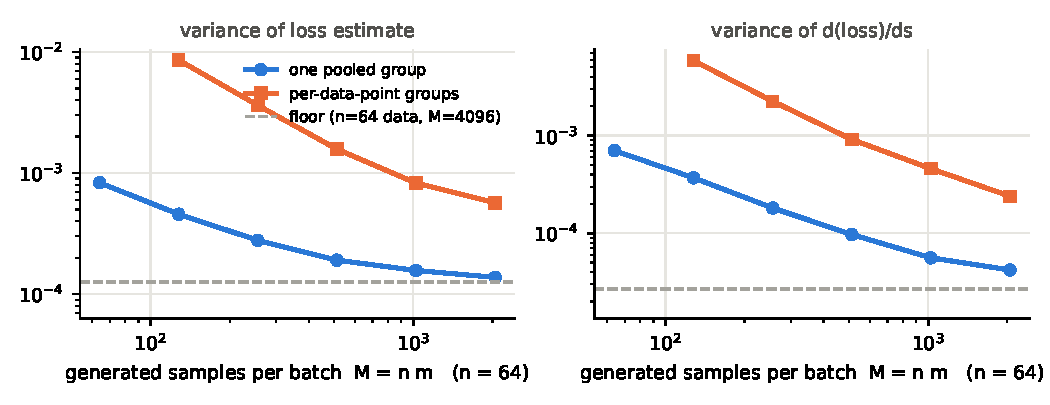
\includegraphics[width=\linewidth]{figures/check_a_variance.pdf}
\caption{Check (a4). Variance vs.\ generated samples per batch $M=nm$ with $n=64$ fixed. Both structures
plateau at the data-only floor (dashed: $M=4096$), as $\sigma_Y^2/n+\tau^2/m$ predicts. At equal $M$, one
pooled group (blue) beats per-data-point groups (orange); for the loss estimate it is up to
\resAfourRatioLoss$\times$ lower.}\label{fig:variance}
\end{figure}

\FloatBarrier
\subsection*{(b) $\beta=2$ cannot separate equal means}
$P=\N(0,1)$, $Q=\N(0,4)$, $n=m=200$, $2000$ replicates. $\widehat D_2$ has mean
$\resBoneDtwoMean\pm\resBoneDtwoSe$ (closed form $0$). $\widehat D_1$ has mean $\resBoneDoneMean\pm\resBoneDoneSe$
(closed form $\resBoneDoneClosed$) and is positive in $\resBoneDoneFracPos\%$ of replicates. A mean shift of
$0.5$ is visible to $\beta=2$: $\widehat D_2$ mean $\resBoneShiftMean$ against $2\cdot0.5^2=0.5$.
Figure~\ref{fig:beta2}, right: expected score minus minimum over $P=\N(0,\sigma^2)$, in closed form using
$\E|\N(0,s^2)|^\beta=s^\beta2^{\beta/2}\Gamma(\tfrac{\beta+1}{2})/\sqrt\pi$. The minimum is at $\sigma=2$ for
every $\beta<2$ and becomes flatter as $\beta\to2$; at $\beta=2$ the curve is identically $0$.
\textbf{(b3)} For $\E|X-Y|-\tfrac\lambda2\E|X-X'|$ over $X\sim\N(0,s^2)$, $Q=\N(0,1)$, the numerical minimiser
matches $s^2=\lambda^2/(2-\lambda^2)$ to $\resBthreeMaxErr$ for $\lambda\in\{0.25,\dots,1.25\}$. For
$\lambda=2$ the loss is $\resBthreeLamTwo$ at $s=1000$, decreasing without bound.
\begin{figure}[htbp]\centering
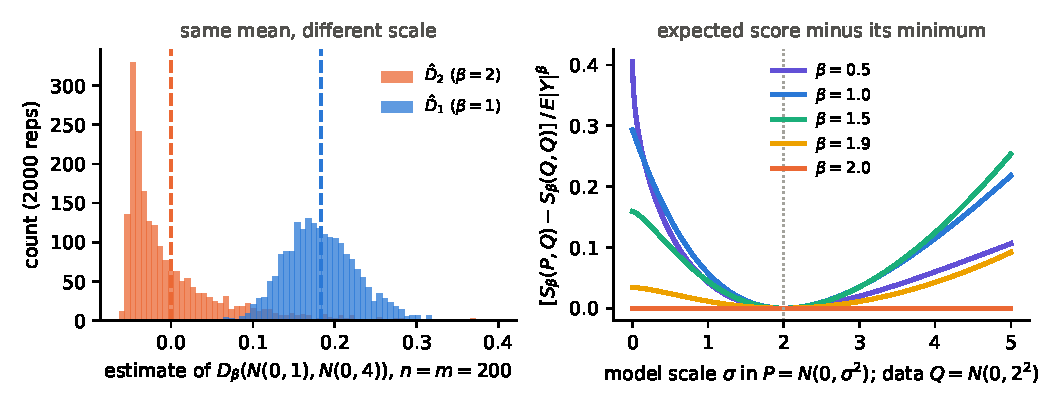
\includegraphics[width=\linewidth]{figures/check_b_beta2.pdf}
\caption{Check (b). Left: $\widehat D_2$ is centred at $0$ although $P\ne Q$; $\widehat D_1$ is centred at the
closed form (dashed). Right: normalised excess expected score; flat for $\beta=2$.}\label{fig:beta2}
\end{figure}

\FloatBarrier
\subsection*{(c) Training a 2-D map with the corrected loss and with readings of the proposed one}
MLP $2\to256\to256\to256\to2$ (SiLU), $z\sim\N(0,I_2)$, target: 8 Gaussians (radius 2, std 0.1). Adam,
learning rate $10^{-3}$ with cosine decay to $0$ (identical for every loss), $3000$ steps, $n=M=256$ per step, $3$ seeds. Metric: $\widehat D_1$ between $4000$
model samples and $4000$ fresh target samples. Reference values: target vs.\ target $\resCbaseTT$; source
Gaussian vs.\ target $\resCbaseGauss$; point mass at the origin (the geometric median) vs.\ target
$\resCbasePoint$.
\begin{table}[htbp]\centering\small
\caption{Check (c): held-out $\widehat D_1$ to the target (mean $\pm$ sd over 3 seeds) and spread of the samples (seed 0).}\label{tab:toy}
\resizebox{\linewidth}{!}{\begin{tabular}{lrrrr}
\toprule
loss & held-out $\widehat D_1$ & sample std (x, y) & mean radius & outside $[-4,4]^2$\\
\midrule
corrected loss, $\beta=1$ & $0.00983\pm5.4\times10^{-4}$ & 1.43, 1.39 & 1.98 & 0\%\\
corrected loss, $\beta=1.5$ & $0.0159\pm0.0011$ & 1.42, 1.41 & 1.97 & 0\%\\
literal: $-\tfrac12\,\texttt{(F(x)-F(x')).mean()}$ & $1.46\pm0.0014$ & 0.00128, 0.00166 & 0.00285 & 0\%\\
$x,x'$ from the data: $-\tfrac12\E\norm{y-y'}$ & $1.46\pm6.4\times10^{-4}$ & 0.000512, 0.00016 & 0.002 & 0\%\\
squared norms in both terms ($\beta=2$) & $1.46\pm0.0029$ & 0.0009, 0.00268 & 0.00247 & 0\%\\
coefficient $1$ instead of $\tfrac12$ & $2.41\times10^{8}\pm7.0\times10^{7}$ & 3.32e+08, 3.38e+08 & 4.09e+08 & 100\%\\
$\norm{\cdot}$, then $-\tfrac12\norm{\cdot}^2$ & $9.65\times10^{8}\pm1.2\times10^{7}$ & 1.06e+09, 1.06e+09 & 1.34e+09 & 100\%\\
\midrule
target (8 Gaussians) & $5.6\times10^{-4}$ & 1.39, 1.44 & 2.00 & 0\%\\
\bottomrule
\end{tabular}
}
\end{table}
\begin{figure}[htbp]\centering
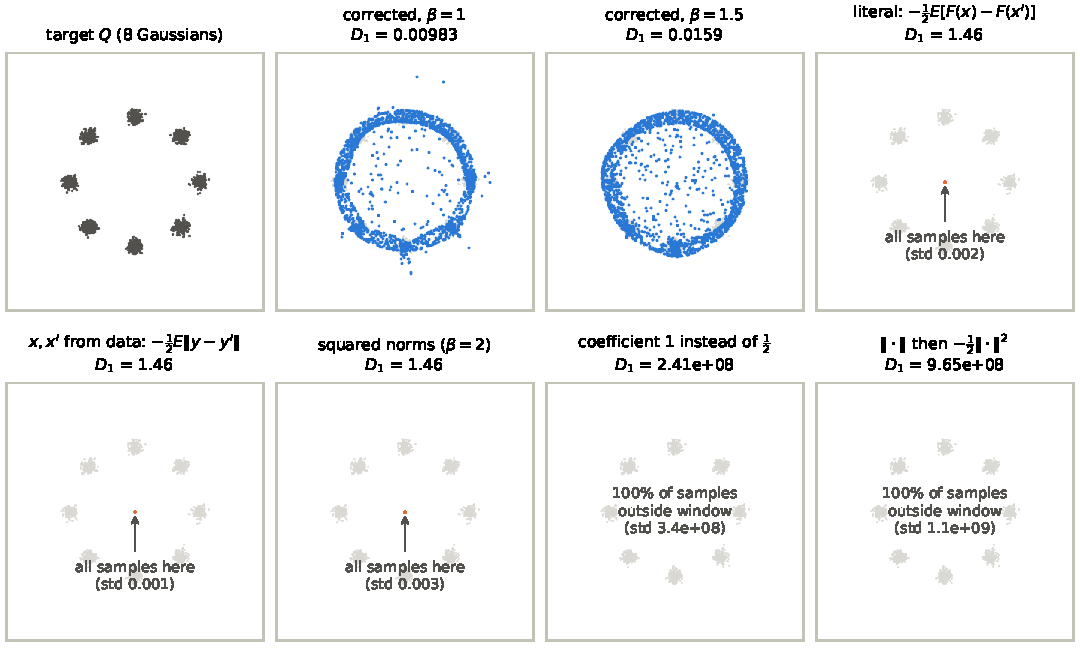
\includegraphics[width=\linewidth]{figures/check_c_samples.pdf}
\caption{Check (c). Samples (seed 0, coloured) over the target (grey). Blue: strictly proper losses.
Orange: readings of the proposed formula. Window $[-4,4]^2$.}\label{fig:toy}
\end{figure}
\begin{figure}[htbp]\centering
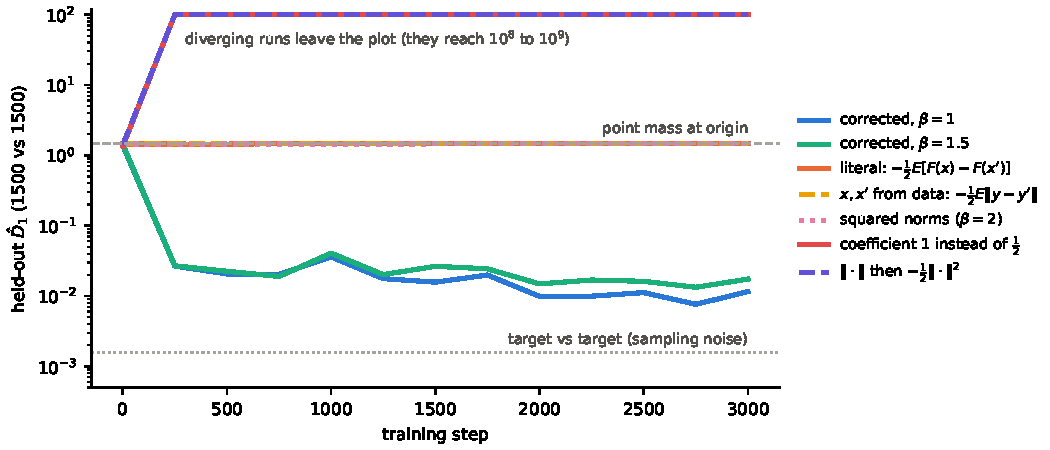
\includegraphics[width=\linewidth]{figures/check_c_curves.pdf}
\caption{Check (c). $\widehat D_1$ to the target during training (seed 0, 1500 vs.\ 1500 samples; values are
clipped to $[10^{-3},10^{2}]$, so negative estimates sit at the bottom and diverging runs at the top).}\label{fig:curves}
\end{figure}

\paragraph{Reading of check (c).} The two strictly proper losses learn the ring and its scale:
$\widehat D_1=\resCesOneDone$ ($\beta=1$) and $\resCesOneHalfDone$ ($\beta=1.5$), against $\resCbaseGauss$ for
the untrained source Gaussian and $\resCbasePoint$ for a point mass. Their sample std, about $1.4$ per
coordinate, matches the target's $\resCTargetStd$. After $3000$ steps, though, the eight modes are only
partly separated: Figure~\ref{fig:toy} shows mass spread along the circle. Check~(c2) (below) shows this is
mainly a training-budget effect. Every reading of the proposed formula fails as Section~\ref{sec:check}
predicts:
\begin{itemize}
\item \emph{Literal} (raw difference, implemented as \texttt{(F(x)-F(x2)).mean()}), \emph{$x,x'$ from the
data}, and \emph{squared norms ($\beta=2$)} all collapse to an almost-point mass near the centre. The sample
std is between $\resCLiteralMinStd$ and $\resCLiteralMaxStd$ for the literal reading, and
$\widehat D_1\approx\resCLiteralDone$ equals the point-mass baseline. For $\beta=2$ the expected loss is
flat in every direction except the mean (Proposition~\ref{prop:beta2}); nothing holds the spread, and in all
three seeds it drifted to a near point mass ($\widehat D_1=\resCBetaTwoDone$).
\item \emph{Coefficient $1$ instead of $\tfrac12$} diverges: the minibatch loss reaches
$\resCCoefOneLossMin$, and the sample std grows to between $\resCCoefOneMinStd$ and $\resCCoefOneMaxStd$
(Proposition~\ref{prop:lambda}(iii)). Growth slows only because the learning rate decays to $0$.
\item \emph{$\norm{\cdot}$ then $-\tfrac12\norm{\cdot}^2$} is unbounded below
(Section~\ref{sec:check}, item~4): minibatch loss down to $\resCMixedLossMin$, $\widehat D_1=\resCMixedDone$.
\end{itemize}


\paragraph{(c2) Longer training.} The corrected loss ($\beta=1$, seed 0), trained the same way for $3000$
and for $20000$ steps. After $3000$ steps, $\widehat D_1=\resCtwoShortDone$ and $\resCtwoShortNear\%$ of
samples lie within $0.3$ (three target standard deviations) of a mode centre. After $20000$ steps,
$\widehat D_1=\resCtwoLongDone$ (below the target-vs-target sampling noise) and the fraction is
$\resCtwoLongNear\%$; the target has $\resCtwoTargetNear\%$. Figure~\ref{fig:long}. The loss does separate
the modes, but the fine structure is learned much more slowly than the coarse structure. That is consistent
with the weight $\norm{t}^{-d-\beta}$ in \eqref{eq:edfourier}, which puts most of $D_\beta$ on low
frequencies. We did not test this explanation further. For images, expect fine detail to converge slowly
(Section~\ref{sec:summary}).
\begin{figure}[htbp]\centering
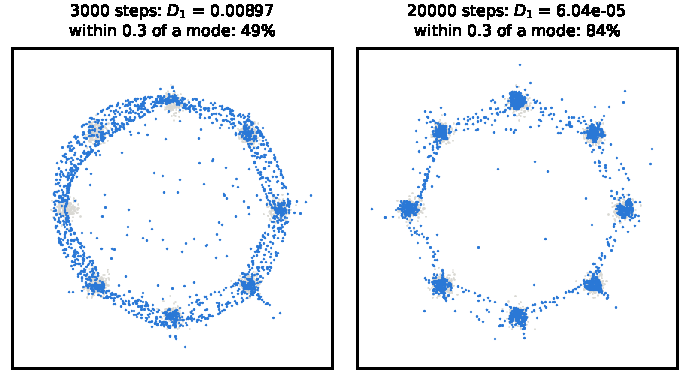
\includegraphics[width=0.62\linewidth]{figures/check_c2_long.pdf}
\caption{Check (c2). Corrected loss, $\beta=1$, seed 0, after $3000$ and $20000$ steps.}\label{fig:long}
\end{figure}

\FloatBarrier
\subsection*{(d) Class-conditional grouping}
This is the example from the proof of Proposition~\ref{prop:pool}: $d=1$, $Q_0=\N(-3,1)$, $Q_1=\N(3,1)$,
$\pi=(\tfrac12,\tfrac12)$, conditional MLP $F(z,\mathrm{onehot}(c))$, $z\sim\N(0,1)$, one generated sample per
data point, $3000$ steps, $2$ seeds. Within the Gaussian family, the pooled loss has derivative
$\resDderivNumeric$ at $s=1$ (numerical), against $(1-e^{-a^2})/(2\sqrt\pi)=\resDderivFormula$. Its minimiser
is $s^\ast=\resDsStar$, close to the $\lambda=\tfrac12$ value $\sqrt{1/7}=\resDlamHalf$. Training gives:
\emph{grouped} (correct) per-class std $\resDgrStdMin$--$\resDgrStdMax$ (target $1$), $\widehat D_1\le\resDgrDoneMax$;
\emph{pooled} (bug) per-class std $\resDpoStdMin$--$\resDpoStdMax$, $\widehat D_1$ between $\resDpoDoneMin$ and
$\resDpoDoneMax$. The pooled model also pushes the class means apart, to $|\text{mean}|$ between
$\resDpoMeanMin$ and $\resDpoMeanMax$ instead of $3$. That is the data-free cross-class repulsion in
Proposition~\ref{prop:pool}; the Gaussian-family calculation held the means fixed, which is why the trained
spread differs from $s^\ast$. Either way the bug gives a wrong minimiser, and the trained model shows it.
Figure~\ref{fig:cond}.

\emph{Secondary 2-D run} (\texttt{check\_d2\_conditional\_2d.py}): two classes on the 8-Gaussian circle,
interleaved (class 0 even modes, class 1 odd modes). $\widehat D_1$ per class, for seed 0 then seed 1:
grouped $\resDtwoDGrDone$; pooled $\resDtwoDPoDone$. Per-coordinate RMS distance to the nearest mode centre
(the target has $\resDtwoDTargetStd$; the bridges between modes inflate it for every model): grouped
$\resDtwoDGrStd$, pooled $\resDtwoDPoStd$. The effect is smaller and seed-dependent here, because with
interleaved classes the cross-class repulsion also depends on within-class spread. We report it for
completeness. The 1-D case is the clean test of Proposition~\ref{prop:pool}.

\begin{figure}[htbp]\centering
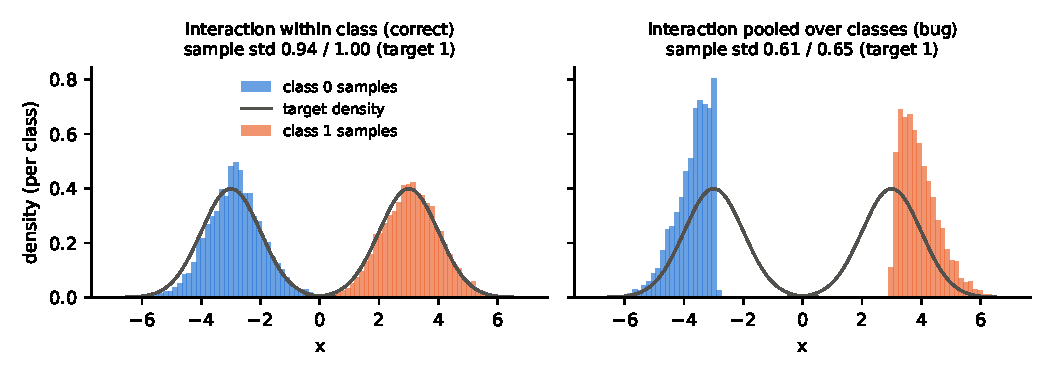
\includegraphics[width=\linewidth]{figures/check_d_conditional.pdf}
\caption{Check (d), seed 0. Per-class histograms of generated samples against the target densities (grey).
Left: interaction term within each class (correct). Right: interaction pooled over all generated pairs
regardless of class (Proposition~\ref{prop:pool}): each class is pushed away from the other and
under-dispersed.}\label{fig:cond}
\end{figure}

\FloatBarrier
\subsection*{(e), (f) Gradient at zero}
\textbf{(e)} PyTorch \resTorchVersion{} on CPU, a $3\times2$ input whose rows~0 and~2 coincide, and the
interaction term computed on the full $3\times3$ matrix with the diagonal masked by multiplication:
\begin{itemize}
\item \texttt{sqrt(((x[:,None]-x[None])**2).sum(-1))} then masking: \texttt{NaN} gradient for every input. The
mask does not help, because $0\cdot\texttt{NaN}=\texttt{NaN}$.
\item \texttt{torch.linalg.vector\_norm} and \texttt{torch.cdist}: finite gradients, $0$ contribution from
zero-distance pairs (\texttt{vector\_norm} of an exact zero vector has gradient $(0,0)$). \texttt{cdist(x,x)**0.5}
was also finite here. Do not rely on this: it holds because \texttt{cdist}'s backward zeroes zero-distance
entries.
\item The double-where distance (\texttt{es\_core.torch\_pow\_dist}): finite for $\beta=0.5,1,1.5$.
\item \texttt{torch.cdist} on $65\times3072$ float32 inputs (matrix-multiplication path) returns diagonal
entries up to $\resEcdistDiag$, and $0.03$ for an exact duplicate pair. With the option
\begin{center}\texttt{compute\_mode="donot\_use\_mm\_for\_euclid\_dist"}\end{center}
they are exactly $0$.
\end{itemize}
\textbf{(f)} The 2-D toy MLP with a zero-initialised last layer, as in DiT, so every generated pair has
distance exactly $0$ at step $0$. With the double-where distance, training is unaffected:
$\resFsafeNaN$ steps with \texttt{NaN} gradients, final $\widehat D_1=\resFsafeDone$. With the naive
\texttt{sqrt}, the gradient is already \texttt{NaN} at the first step, $\resFnaiveSteps$ of $3000$ steps have
\texttt{NaN} gradients, and the trained model outputs \texttt{NaN}: once a \texttt{NaN} reaches the Adam
state, the parameters are lost.


%======================================================================
\section{Summary for the next stages}\label{sec:summary}
\begin{itemize}
\item \textbf{Loss:} \eqref{eq:final} with $\beta=1$: confinement $\norm{F_\theta(Z,C)-Y}$ minus $\tfrac12$
interaction $\norm{F_\theta(Z,C)-F_\theta(Z',C)}$, with $Z,Z'$ i.i.d.\ $\N(0,I)$, independent of the data,
and \emph{the same class} in both interaction arguments.
\item \textbf{Estimator:} \eqref{eq:estimator}, grouping by class within the batch, weights $n_c/N$,
$m_c\ge2$, diagonal excluded (U-statistic), double-where norm.
\item \textbf{Metric:} per-class held-out $\widehat D_1$ (unbiased; can be $<0$ on a batch).
\item \textbf{Watch for:} \texttt{NaN} at step $0$ with DiT's zero-initialised head if the norm is computed
naively; V-statistic bias with small $m_c$; pooling the interaction across classes.
\end{itemize}
\paragraph{Open questions.} (1) $\beta=1$ versus $\beta\in(1,2)$ on images: both are strictly proper;
$\beta=1$ is standard (engression, CRPS), and De Bortoli et al.\ report results over a range of $\beta$
\cite{DeBortoli2025}. Untested here. (2) Pixel space versus latent space: the theory is the same, but the
Euclidean norm on pixels is a poor perceptual metric, and the energy distance in high dimension may be
dominated by low-frequency or mean differences. This is the main practical risk for the one-step image test
(stage~2 decides). Check~(c2) points the same way: in 2-D the energy score learned coarse structure in a
few hundred steps but needed about $20000$ steps to separate the modes. (3) How small the per-class $m_c$ can be at DiT scale without the variance hurting;
check~(a4) suggests $m_c=n_c$ with per-class pooling is enough to reach the data-noise floor.

%======================================================================
\begingroup\raggedright
\begin{thebibliography}{99}
\bibitem{GR2007} T.~Gneiting and A.~E. Raftery. Strictly proper scoring rules, prediction, and estimation.
\emph{Journal of the American Statistical Association} 102(477):359--378, 2007.
\href{https://doi.org/10.1198/016214506000001437}{doi:10.1198/016214506000001437}. Text checked:
\url{https://sites.stat.washington.edu/raftery/Research/PDF/Gneiting2007jasa.pdf} (Secs.~1--2, eqs.~(1), (2), (7), (22)--(24); Sec.~5.1, Thm.~4, Ex.~9).
\bibitem{SR2013} G.~J. Sz\'ekely and M.~L. Rizzo. Energy statistics: A class of statistics based on distances.
\emph{Journal of Statistical Planning and Inference} 143(8):1249--1272, 2013.
\href{https://doi.org/10.1016/j.jspi.2013.03.018}{doi:10.1016/j.jspi.2013.03.018}. Text checked:
\url{https://pages.stat.wisc.edu/~wahba/stat860public/pdf4/Energy/JSPI5102.pdf} (Def.~1, Props.~1--2, eqs.~(2.6), (5.1), (5.2), Lemma~1, App.~A).
\bibitem{Sejdinovic2013} D.~Sejdinovic, B.~Sriperumbudur, A.~Gretton and K.~Fukumizu. Equivalence of
distance-based and RKHS-based statistics in hypothesis testing. \emph{Annals of Statistics} 41(5):2263--2291, 2013.
\href{https://doi.org/10.1214/13-AOS1140}{doi:10.1214/13-AOS1140}; \url{https://arxiv.org/abs/1207.6076} (Def.~13, Thm.~22).
\bibitem{SM2025} X.~Shen and N.~Meinshausen. Engression: extrapolation through the lens of distributional
regression. \emph{Journal of the Royal Statistical Society Series B} 87(3):653--677, 2025.
\href{https://doi.org/10.1093/jrsssb/qkae108}{doi:10.1093/jrsssb/qkae108}; \url{https://arxiv.org/abs/2307.00835} (v3: eqs.~(8), (12), (13); App.~E).
\bibitem{DeBortoli2025} V.~De Bortoli, A.~Galashov, J.~S. Guntupalli, G.~Zhou, K.~Murphy, A.~Gretton and
A.~Doucet. Distributional diffusion models with scoring rules. ICML 2025 (PMLR 267).
\url{https://arxiv.org/abs/2502.02483} (v3: eqs.~(8), (12), (13), Prop.~4.1).
\bibitem{Shen2025RML} X.~Shen, N.~Meinshausen and T.~Zhang. Reverse Markov learning: multi-step generative
models for complex distributions. arXiv:2502.13747, 2025. \url{https://arxiv.org/abs/2502.13747}.
\bibitem{Bellemare2017} M.~G. Bellemare, I.~Danihelka, W.~Dabney, S.~Mohamed, B.~Lakshminarayanan, S.~Hoyer and
R.~Munos. The Cram\'er distance as a solution to biased Wasserstein gradients. arXiv:1705.10743, 2017.
\url{https://arxiv.org/abs/1705.10743}.
\bibitem{Li2015} Y.~Li, K.~Swersky and R.~Zemel. Generative moment matching networks. arXiv:1502.02761, 2015.
\url{https://arxiv.org/abs/1502.02761}.
\bibitem{Gritsenko2020} A.~A. Gritsenko, T.~Salimans, R.~van den Berg, J.~Snoek and N.~Kalchbrenner. A spectral
energy distance for parallel speech synthesis. arXiv:2008.01160, 2020. \url{https://arxiv.org/abs/2008.01160}.
\bibitem{DiTcode} W.~Peebles and S.~Xie. DiT reference code, \texttt{models.py},
\texttt{initialize\_weights}. \url{https://github.com/facebookresearch/DiT/blob/ed81ce2229091fd4ecc9a223645f95cf379d582b/models.py}.
\end{thebibliography}
\endgroup
\end{document}
